\section{SAT and CNF-SAT}

\subsection{Formula Satisfiability/SAT}
$(a \vee b \vee c \vee \overbar{d})$ <=>  $((b \wedge \overbar{c}) \vee \overbar{ ( \overbar{a} => d) } \vee (c \neq a \wedge b)) $

\subsection{CNF}
conjunction/AND of several clauses which use OR inside these clauses.
\subsection{3CNF}
cnf with exactly 3 literals per clause

\subsection{Maximum Independent Set (from 3Sat)}
input is a simple, unweighted graph, get the size of the largest/smallest subgraph
Make the formula into a graph or vice versa, if it has an independent set of size $k$, its possible
Any graph has an edge-complement with the same vertices but the opposite set of edges if its not an edge in $G$. Its independent in $G$ if and only if the same vertices define a clique in $\overbar{G}$ (a complete graph). The largest independent is thus the largest clique in the compliment of the graph.

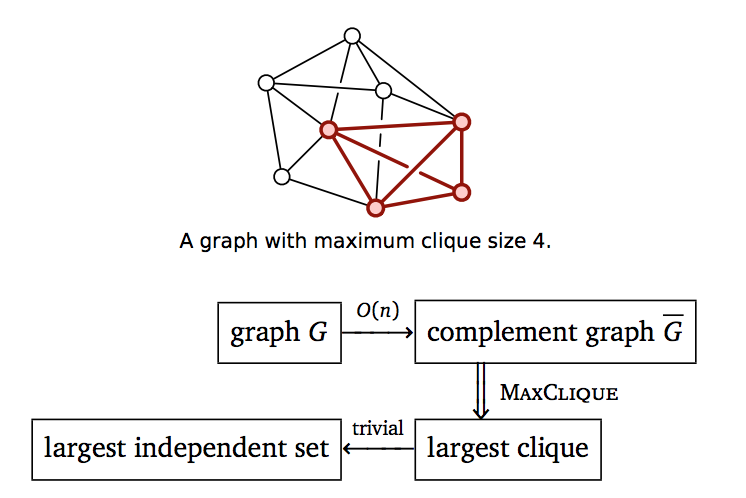
\includegraphics[width=\linewidth]{images/maxclique.png}

\subsection{3Color [From 3SAT]}
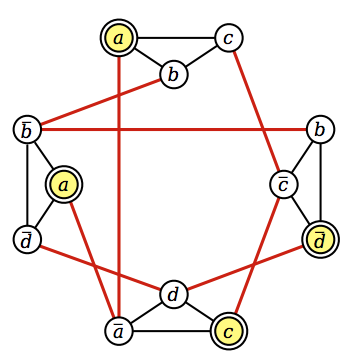
\includegraphics[width=\linewidth]{images/hamcycle.png}
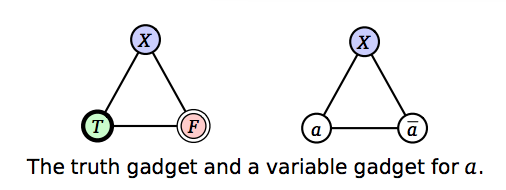
\includegraphics[width=\linewidth]{images/truthgadget.png}
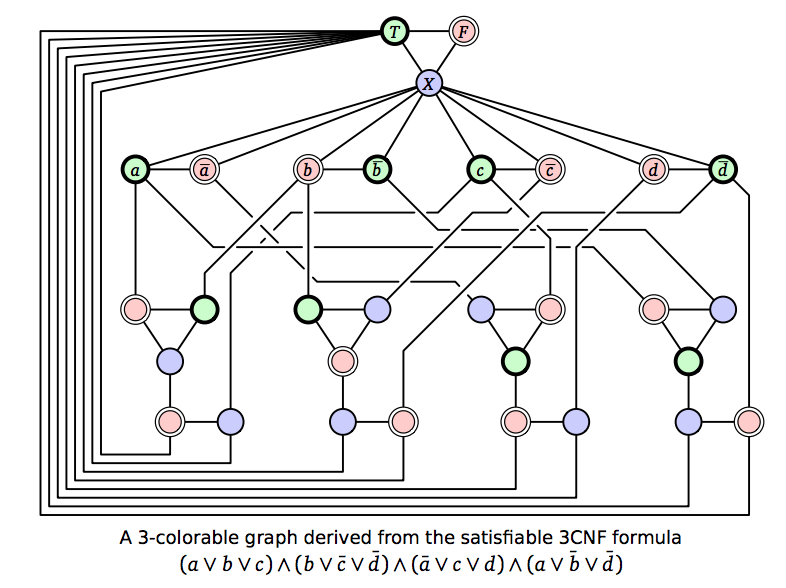
\includegraphics[width=\linewidth]{images/3color.png}

Truth gadget: $T,F$, and $X$ for true/false/other, variable gadget for variable a connecting and $\overbar{a}$ which must be opposite bools. Clause gadget joining three literal nodes to node $T$ in the truth gadget using give new unlabeled nodes and ten edges.